% Anonymous ICASSP draft. Compile from paper/ with IEEEtran available.
\documentclass[conference]{IEEEtran}
\usepackage{graphicx}
\usepackage{amsmath}
\usepackage{amssymb}
\usepackage{booktabs}
\graphicspath{{figures/}}

\title{CARE: Repair Before You Decide in Lossy Multi-Robot Map Sharing}
\author{Anonymous Authors}

\begin{document}
\maketitle

\begin{abstract}
A dropped occupancy update matters only if it leaves a robot unable to choose
an imminent action. We introduce CARE, a replica-repair protocol that turns
this observation into a finite encoded-byte optimization. For up to eight
path-near uncertain cells, CARE enumerates all occupancy scenarios with at most
two blocked cells, retains action-conflicting pairs whose first divergence is
no earlier than the measured query--patch round trip, and computes an exact
minimum encoded-query-size hitting set separating those pairs. On 100 matched controlled
maps with 5$\times$5 sensing and 30\% packet loss, CARE raises decision-critical
seeker completion from .3425 to .4725 with A* and from .3800 to .5375 with D*
Lite, for 5.63/5.47~KB beyond one-shot sharing. Codec-matched adaptations of
forward simulation, path-guided compression, rate--distortion allocation and
value-of-information routing show a narrower result: CARE is not uniformly
more reliable; several paired intervals include zero, while CARE uses about 9.5~KB less than
the path-guided and rate--distortion adaptations. A separate natural-map suite
does not detect a broad CARE--one-shot reliability gain. A 1,600-episode
negative ablation also rejects an auxiliary route-slack gate. CARE therefore
provides an exact certificate inside a declared bounded uncertainty model, not
a universal communication advantage.
\end{abstract}

\begin{IEEEkeywords}
multi-robot systems, map sharing, lossy communication, replica repair,
decision certificates
\end{IEEEkeywords}

\section{Introduction}
Multi-robot systems often exchange explicit occupancy cells while each robot
plans on a private, initially unknown replica. Packet loss can make replicas
disagree, yet repairing every disagreement is wasteful: most stale cells do
not alter the next route decision. Conventional choices span no communication,
retrying every update, and periodic full anti-entropy. They answer how to
reconcile state, but not the decision question: \emph{which cells must arrive
before the receiver can still change action?}

We study that question without learning a motion policy. DCC and SCRIMP learn
communication inside different MAPF representations
\cite{ma2021dcc,wang2023scrimp}; they are related systems, not codec-matched
replica-repair baselines. Distributed anti-entropy instead advances version
vectors, localizes differences with Merkle trees, or decodes set differences
\cite{vanrenesse2008scuttlebutt,decandia2007dynamo,goodrich2011iblt}.
Communication-aware robotics has also optimized future communication by
forward simulation \cite{marcotte2020ocbc}, compressed maps around paths
\cite{psomiadis2023compression}, allocated bits using rate--distortion
\cite{psomiadis2025ratedistortion}, and routed information by utility
\cite{barcis2021utility}. Their original states and messages differ from our
exact-cell query--patch protocol; we therefore compare declared, codec-matched
\emph{inspired adaptations}, not claim exact reproductions.

CARE's contribution is a bounded joint-scenario decision certificate. First,
it prices queries with the executable wire codec. Second, it uses the first
action divergence of each conflicting scenario pair as that pair's repair
deadline. Third, it solves a uniform-byte minimum hitting set exactly. We
evaluate both A* and D* Lite with paired map-cluster inference. Crucially, we
also report where the result fails to generalize: the controlled maps share a
fixed decision structure; natural non-tiled maps show no broad gain; and an
extra route-slack gate is empirically harmful and excluded from final CARE.

\section{CARE: A Minimum Decision Certificate}
Robot $i$ maintains a versioned occupancy replica $M_i^t$. Observations create
directed one-shot deltas, and an incoming cell is merged only when its
deterministic stamp dominates the local copy. Data, query and patch packets
share the same lossy/delayed channel and byte caps. A cell delta is 13 bytes; a
query over $m$ stamped cells costs $16+6m$ bytes; and a returned patch costs
$4+13m$ bytes. Attempted traffic includes dropped packets.

For receiver $j$, let $U_j$ contain at most $n=8$ UNKNOWN cells on, or one
graph hop from, the next $H=8$ optimistic path vertices. A scenario
$\omega\subseteq U_j$ marks blocked candidates. CARE declares the bounded
family
\begin{equation}
 \Omega_q(U_j)=\{\omega\subseteq U_j:|\omega|\le q\},\qquad q=2,
\end{equation}
so at most $S=\sum_{r=0}^{q}\binom{n}{r}=37$ scenarios are replanned on the
same four-neighbor action graph. Let $\pi_\omega$ be a canonical path and let
$\delta(\omega,\omega')$ be the first action at which two paths diverge. For
one-way link delay $d$, the measured request--response time is
$L_{\rm rtt}=2d$. Final CARE retains the conflict
$e=(\omega,\omega')$ only when $\pi_\omega\ne\pi_{\omega'}$ and
$\delta(\omega,\omega')\ge L_{\rm rtt}$. Its distinguishability set is
$D_e=\omega\triangle\omega'$. CARE then solves
\begin{equation}
 \min_{Q\subseteq U_j}16+6|Q|\quad
 \text{s.t. }Q\cap D_e\neq\varnothing,\quad\forall e\in\mathcal E_j .
 \label{eq:certificate}
\end{equation}

\textit{Proposition.} If the requested binary cell states are returned, a
query $Q$ identifies every deadline-feasible action class in $\Omega_q$ iff it
satisfies (\ref{eq:certificate}).

\textit{Proof.} Two scenarios return the same binary query signature exactly
when $Q$ misses their symmetric difference. Missing any action-conflicting
$D_e$ therefore leaves two feasible actions indistinguishable; hitting all of
them separates every such pair. Because every query entry costs six bytes, a
minimum-cardinality hitting set is also minimum encoded query size. \hfill$\Box$

Cardinality-ordered subset enumeration is exact within the declared caps, with
cost $O(SP+S^2H+2^n|\mathcal E_j|n)$ for bounded path-search cost $P$. This is
not a guarantee for arbitrary map uncertainty, and a queried peer need not
know every requested cell. Importantly, final CARE contains no additional
optimistic/pessimistic route witness. The action-divergence filter above is its
only deadline mechanism.

\section{Experimental Design}
All methods use identical maps, local sensing, A*/D* Lite interfaces, packet
traces, delay, wire codec and byte accounting. The controlled task has four
remote observers paired with four decision-critical seekers. Observers start
one step from their goals and succeed in every audited controlled run; hence
all-robot completion has a structural .5 floor and is only diagnostic:
\begin{equation}
 \mathrm{CSR}_{\rm all}=(1+\mathrm{CSR}_{\rm seeker})/2.
\end{equation}
Our primary endpoint is seeker CSR. We report mean episode length (EL),
attempted KB, and 20,000-draw bootstrap 95\% confidence intervals (CIs) that
resample whole maps through one fixed public resampling index. Differences are
paired within the same map and loss trace.

The primary 5$\times$5, 30\%-loss point uses 100 controlled maps. They are
independent background-clutter realizations under one protected multifork
decision template, not 100 independent task structures. Main, loss, sensing,
delay, ablation, topology and baseline studies total 69,800 executions,
including repeated anchors; this is a run count, not an independent-sample
count. The older 4--32-agent extension tiles the same fork motif and is only a
load stress test.

Baselines span one-shot delivery, Retry-All ARQ, Periodic Full Sync and
task-aware Path-Aware Top-K and Single-Cell Sensitivity. The closest-work suite
adds four exact-cell adaptations: OCBC-style forward simulation (OCBC-FS),
path-guided spatial coverage (PGSC), Bernoulli rate--distortion allocation
(BRD), and VoI per encoded byte. Their query--patch codec, loss trace and cap
match CARE; their scores do not use CARE's joint hitting-set certificate.
All blocked counterfactuals use canonical A* on the common unit-cost graph,
while the executed planner is independently A* or D* Lite.

External validity is tested on 100 immutable Bernoulli maps conditioned, before
any policy runs, on a frozen action-conflict, visibility, path-length,
communication-window and disjointness predicate bundle. A
separate non-tiled scale study uses 100 maps at each of 4, 8, 16 and 32 agents.
Finally, a 1,600-execution negative ablation studies two \emph{non-final}
route-witness variants: a first-UNKNOWN route-slack hard gate and the identical
witness without that gate.

\section{Results}
\subsection{Controlled reliability--traffic result}
Table~\ref{tab:primary} reports the direct role-aware endpoint. CARE improves
over One-shot by $+.1300$ (paired CI $[+.1000,+.1625]$) with A* and $+.1575$
($[+.1225,+.1925]$) with D* Lite, for only 5.63/5.47~KB. Retry-All remains the
higher-reliability endpoint: CARE is lower by $.0450/.0350$ while saving
101.20/101.75~KB. EL is 25 throughout because the controlled horizon is
censored at 25; no speed claim follows from it.

\begin{table}[t]
\caption{Controlled primary point: seeker CSR mean [95\% CI], mean EL, and
attempted KB; 100 matched maps, 5$\times$5 sensing, 30\% loss.}
\label{tab:primary}
\centering
\scriptsize
\resizebox{\columnwidth}{!}{%
\begin{tabular}{lccc ccc}
\toprule
& \multicolumn{3}{c}{A*} & \multicolumn{3}{c}{D* Lite}\\
\cmidrule(lr){2-4}\cmidrule(lr){5-7}
Method & Seeker CSR [CI] & EL & KB & Seeker CSR [CI] & EL & KB\\
\midrule
One-shot & .3425 [.3025,.3825] & 25 & 47.62 & .3800 [.3375,.4225] & 25 & 47.78\\
Retry-All & .5175 [.4825,.5525] & 25 & 154.45 & .5725 [.5400,.6050] & 25 & 155.00\\
Path Top-K & .4550 [.4200,.4900] & 25 & 54.37 & .5225 [.4850,.5600] & 25 & 54.39\\
Single-Cell & .4650 [.4300,.5000] & 25 & 52.11 & .5250 [.4900,.5600] & 25 & 52.23\\
OCBC-FS$^\dagger$ & .4725 [.4375,.5075] & 25 & 52.57 & .5350 [.5000,.5700] & 25 & 52.54\\
PGSC$^\dagger$ & .4800 [.4425,.5150] & 25 & 62.79 & .5350 [.4975,.5725] & 25 & 62.87\\
BRD$^\dagger$ & .4800 [.4450,.5150] & 25 & 62.74 & .5350 [.4975,.5700] & 25 & 62.88\\
CARE & .4725 [.4350,.5075] & 25 & 53.25 & .5375 [.5000,.5750] & 25 & 53.25\\
\bottomrule
\multicolumn{7}{l}{\scriptsize $^\dagger$Codec-matched inspired adaptation, not exact reproduction.}
\end{tabular}
}
\end{table}

The closest comparisons delimit the novelty. CARE--Path Top-K is $+.0175$
($[+.0025,+.0325]$) with A* and $+.0150$ ($[.0000,+.0300]$) with D* Lite,
while CARE sends 1.12/1.13~KB less. Against Single-Cell, the differences are
$+.0075$ ($[-.0075,+.0250]$) and $+.0125$ ($[-.0025,+.0300]$), while CARE
sends 1.14/1.03~KB more. No CARE--OCBC-FS reliability difference is detected.
The CARE--PGSC and CARE--BRD paired intervals also include zero, while CARE
saves about 9.5~KB. Against VoI-per-byte, the differences are $+.0125$
($[-.0025,+.0275]$) and $+.0050$ ($[-.0150,+.0225]$), while CARE sends
.76/.69~KB more. Thus the evidence does not support universal reliability
dominance; it supports a compact exact certificate relative to broader path
allocation.

\begin{figure}[t]
 \centering
 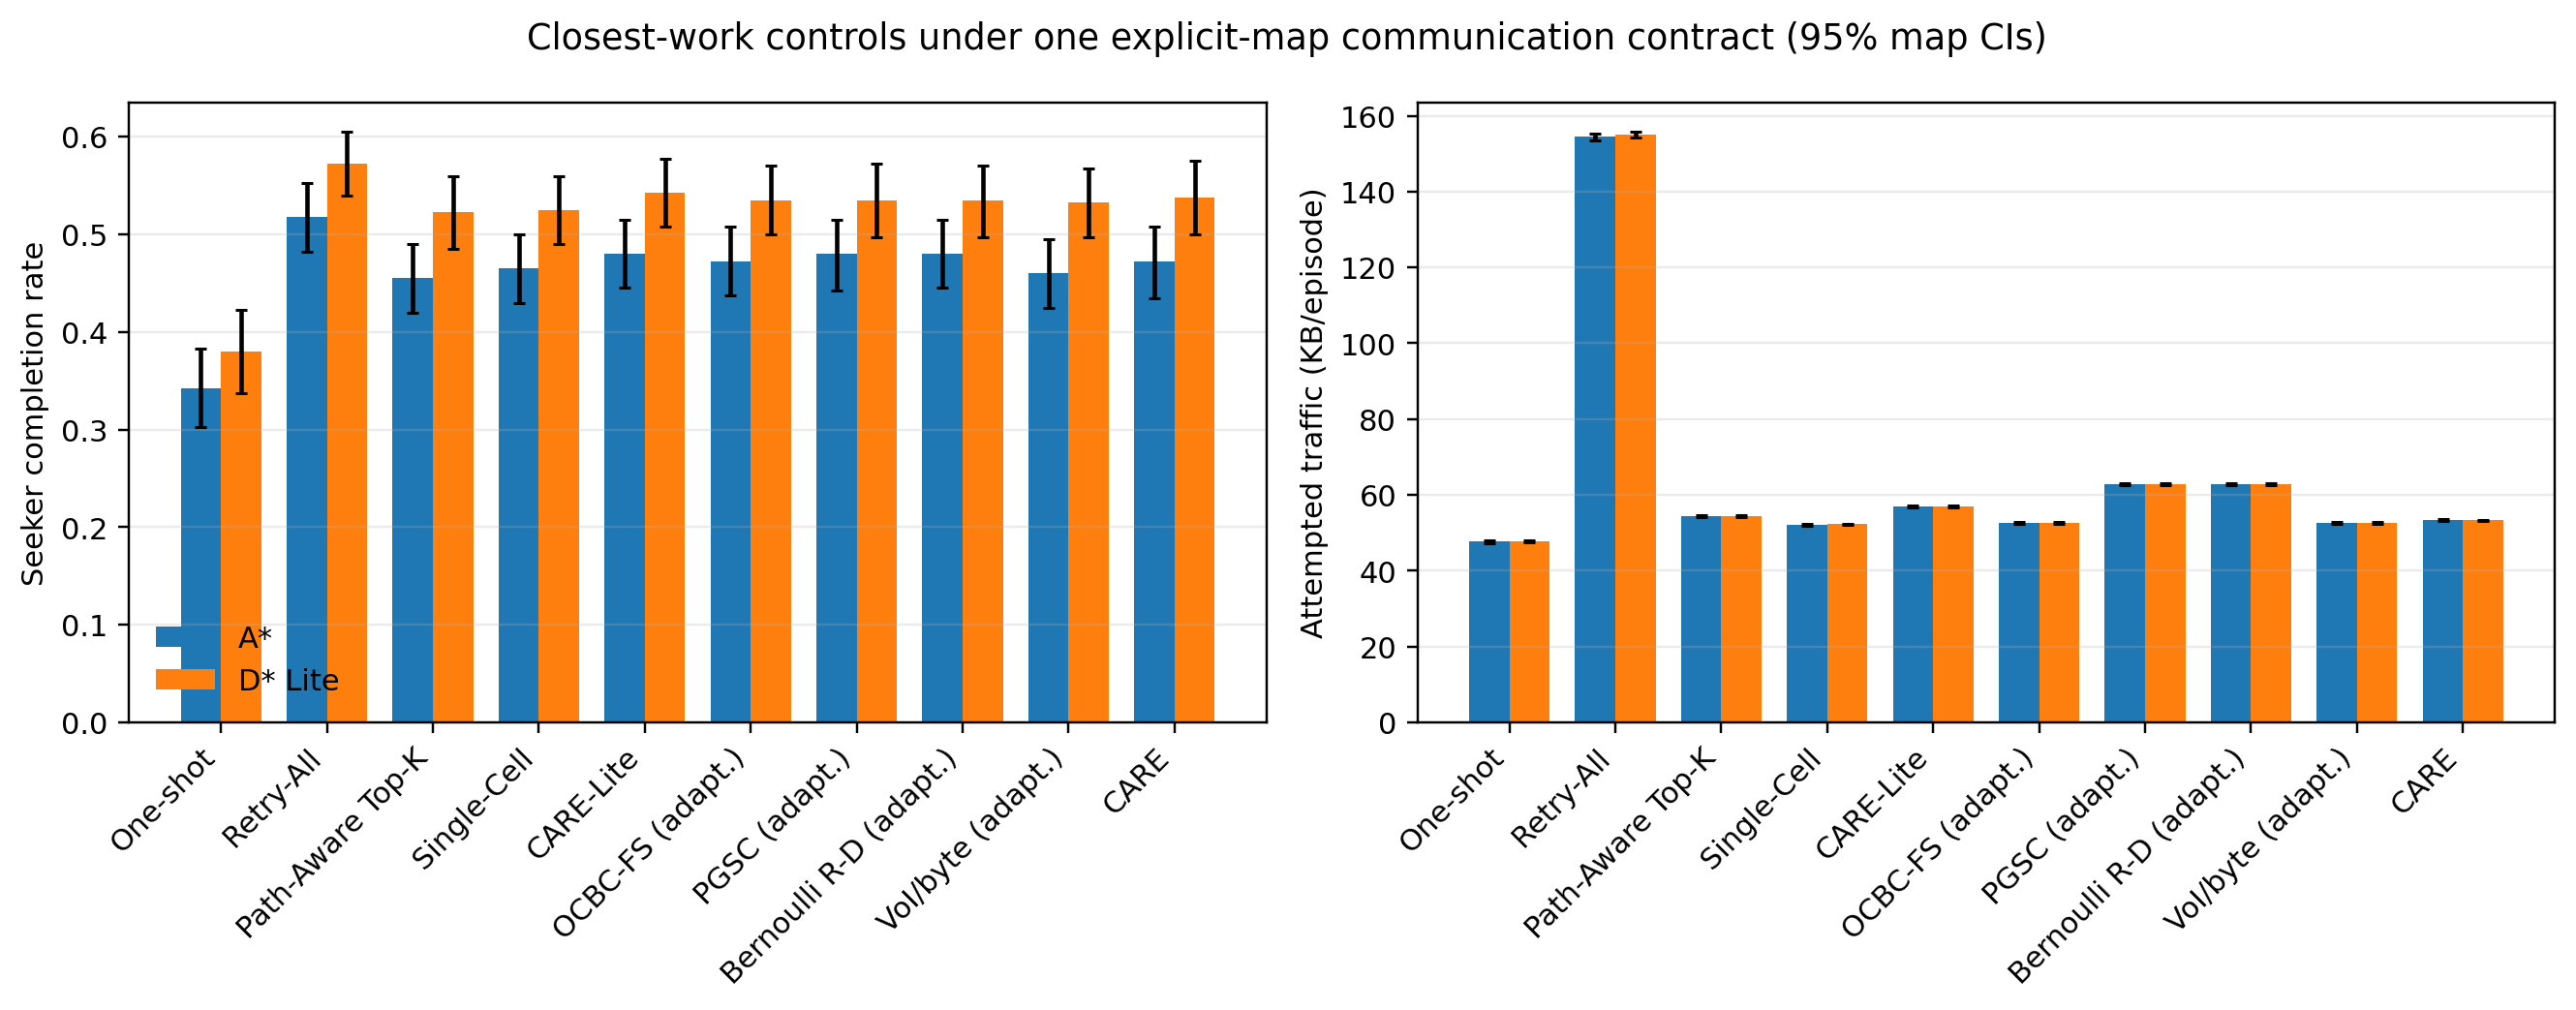
\includegraphics[width=\columnwidth]{care_closest_work.png}
 \caption{Codec-matched closest-work controls at the controlled 5$\times$5,
 30\%-loss point. Error bars are seeker-CSR map-bootstrap 95\% CIs; the right
 panel reports attempted KB per episode.}
 \label{fig:closest}
\end{figure}

\begin{figure}[t]
 \centering
 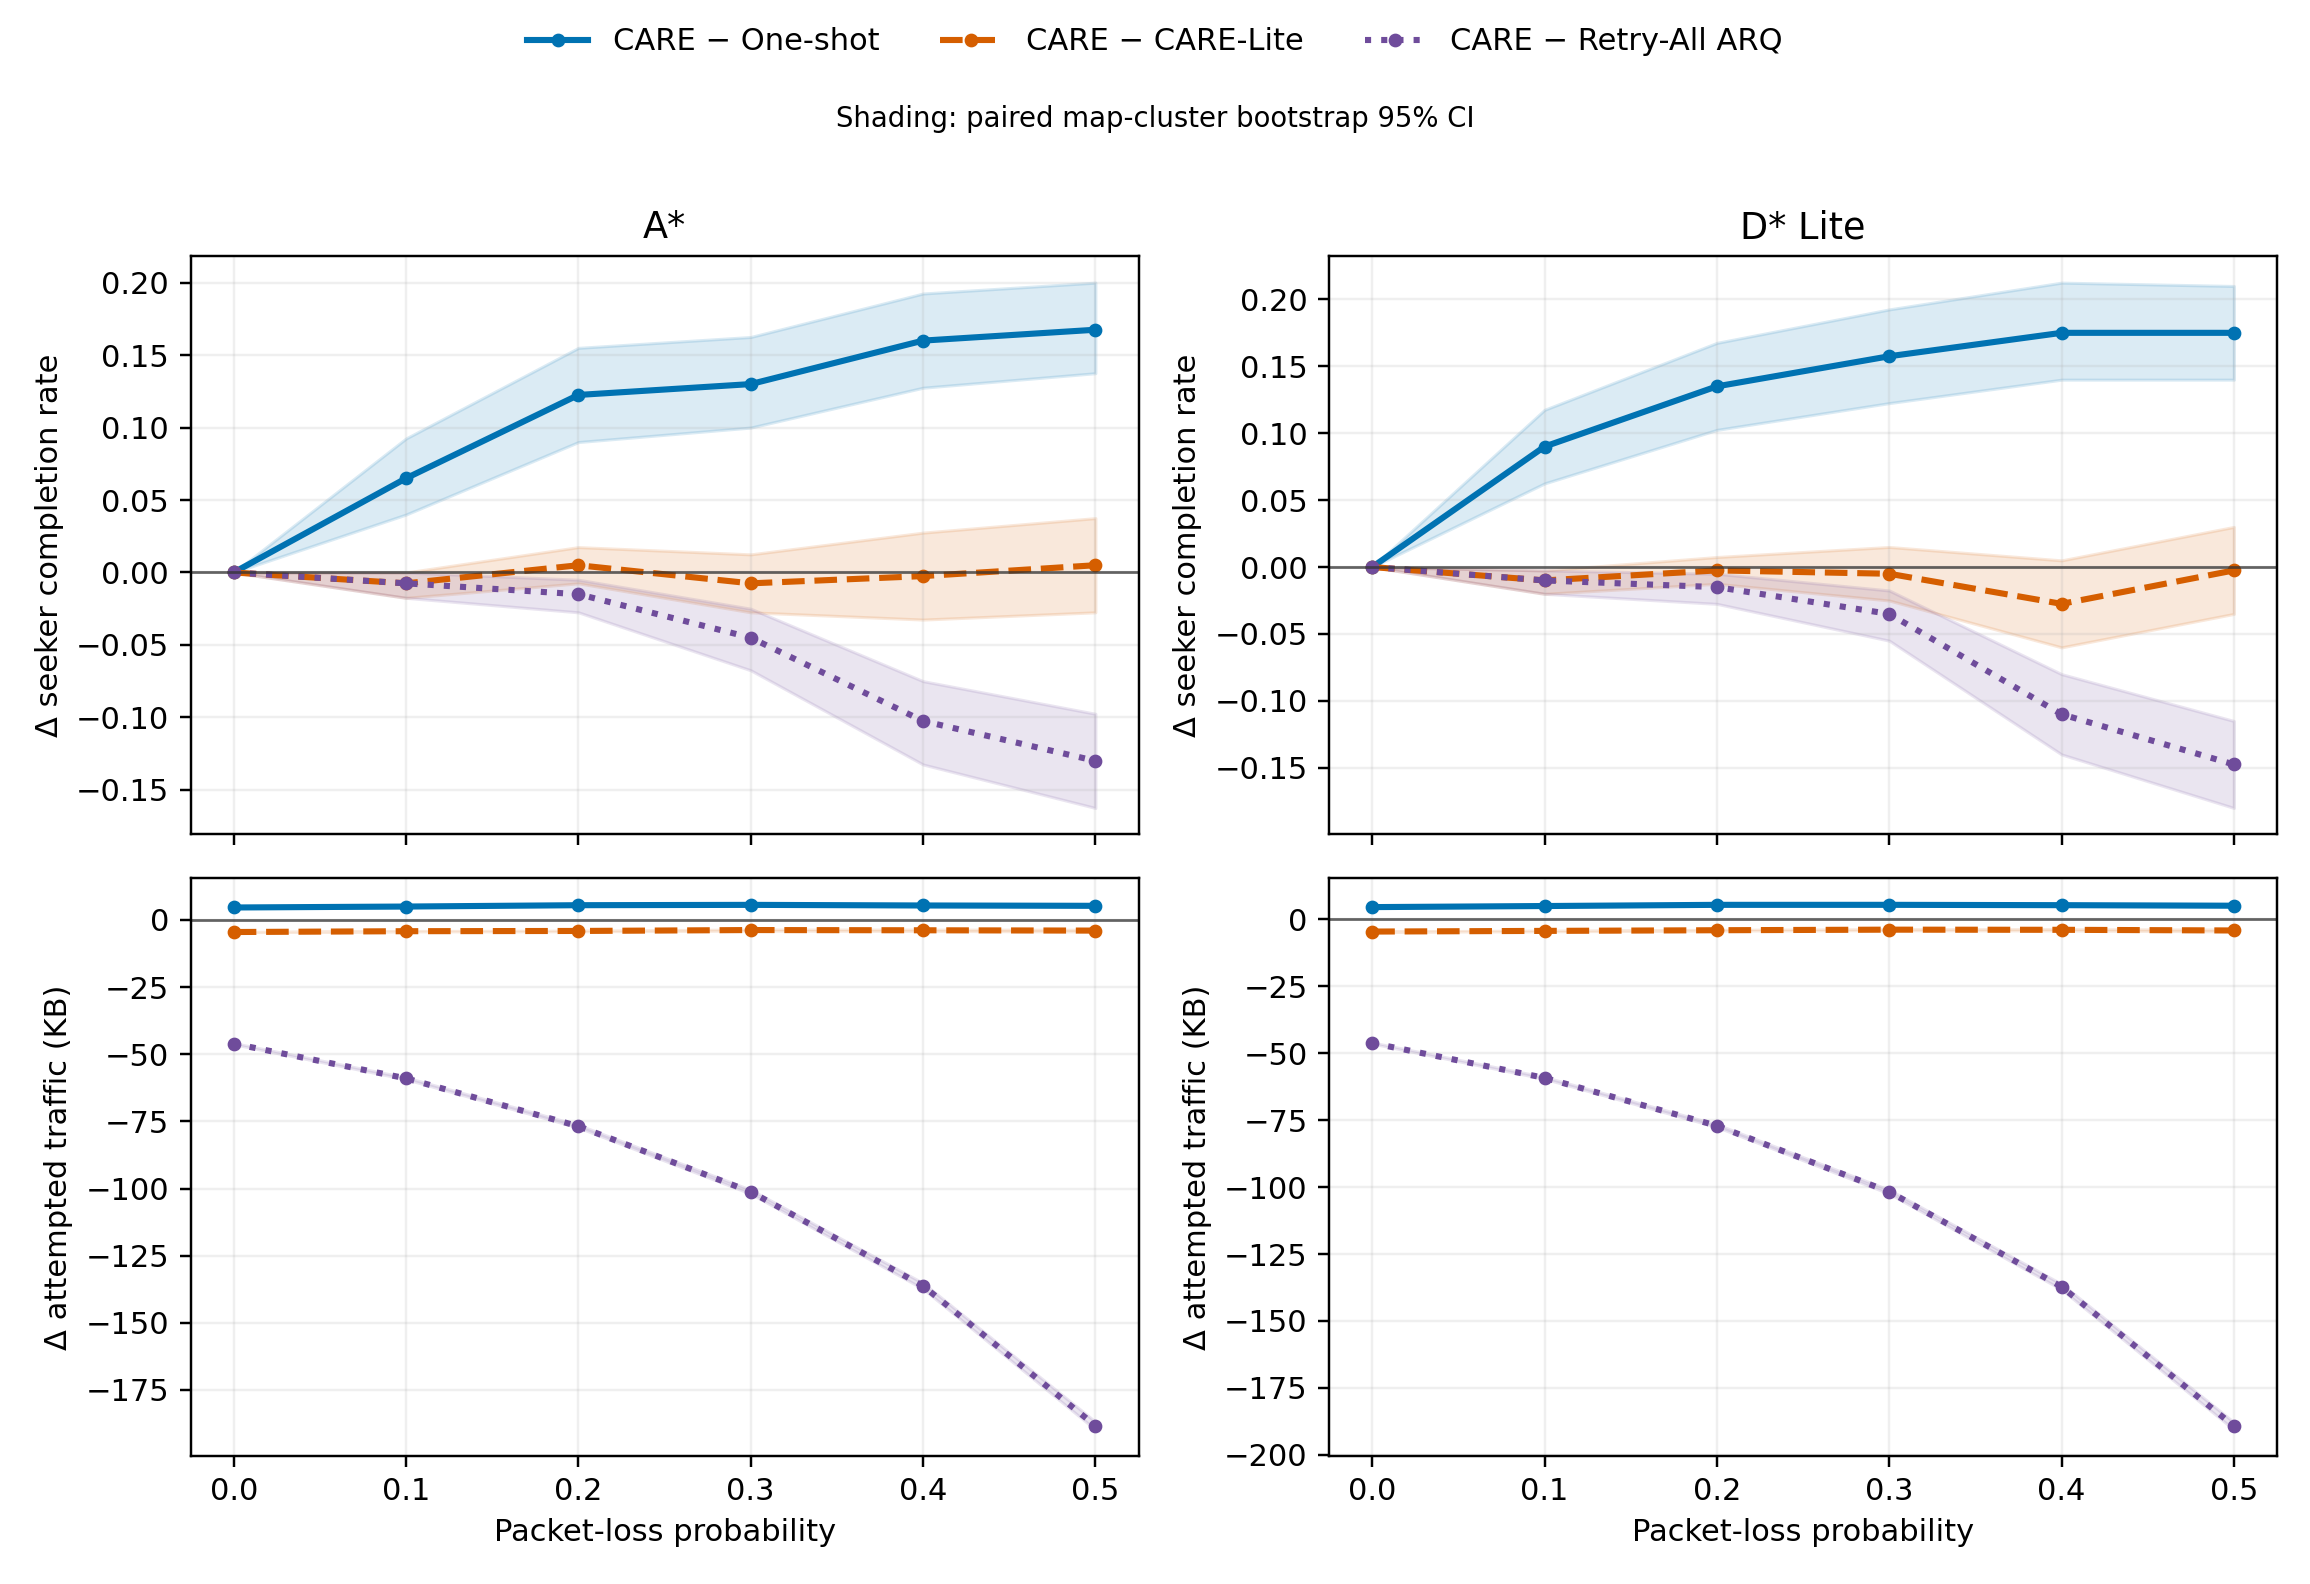
\includegraphics[width=\columnwidth]{care_loss_baseline_sweep.png}
 \caption{Paired CARE-minus-comparator seeker-CSR and attempted-traffic
 differences across loss rates. Every subtraction matches the same map and
 loss trace; shading is the paired map-cluster bootstrap 95\% CI. Reliable ARQ
 remains the higher-traffic reliability endpoint.}
 \label{fig:loss}
\end{figure}

\subsection{Deadline ablation and external validity}
The auxiliary route-witness experiment is a negative result. At two-step
one-way delay, gating that witness reduces seeker success relative to the
ungated witness by $.0525$ (CI $[.0325,.0725]$) with A* and $.0575$
($[.0375,.0800]$) with D* Lite, although it saves about 6.1~KB. At delay four,
it saves 12.64~KB without a detected success change. This does not establish
incremental commitment-gate value; neither witness variant is final CARE.
The retained deadline rule is only pairwise action-divergence feasibility in
(\ref{eq:certificate}).

The natural conditioned-random suite sharply narrows the generality claim.
CARE--One-shot is $+.0050$ ($[-.0050,+.0150]$) with A* and $-.0025$
($[-.0125,+.0075]$) with D* Lite. CARE--No Communication is likewise
inconclusive: $+.0200$ ($[-.0050,+.0450]$) and $+.0175$
($[-.0075,+.0450]$). With D* Lite, CARE--Periodic Full is $-.0125$
($[-.0275,-.0025]$) while CARE sends about 361~KB less. Across non-tiled natural
4/8/16/32-agent studies, every paired CARE--One-shot seeker-CI crosses zero.
Consequently the controlled result demonstrates the mechanism under protected
decision-critical loss; it is not evidence of a broad gain on arbitrary maps.

\begin{figure}[t]
 \centering
 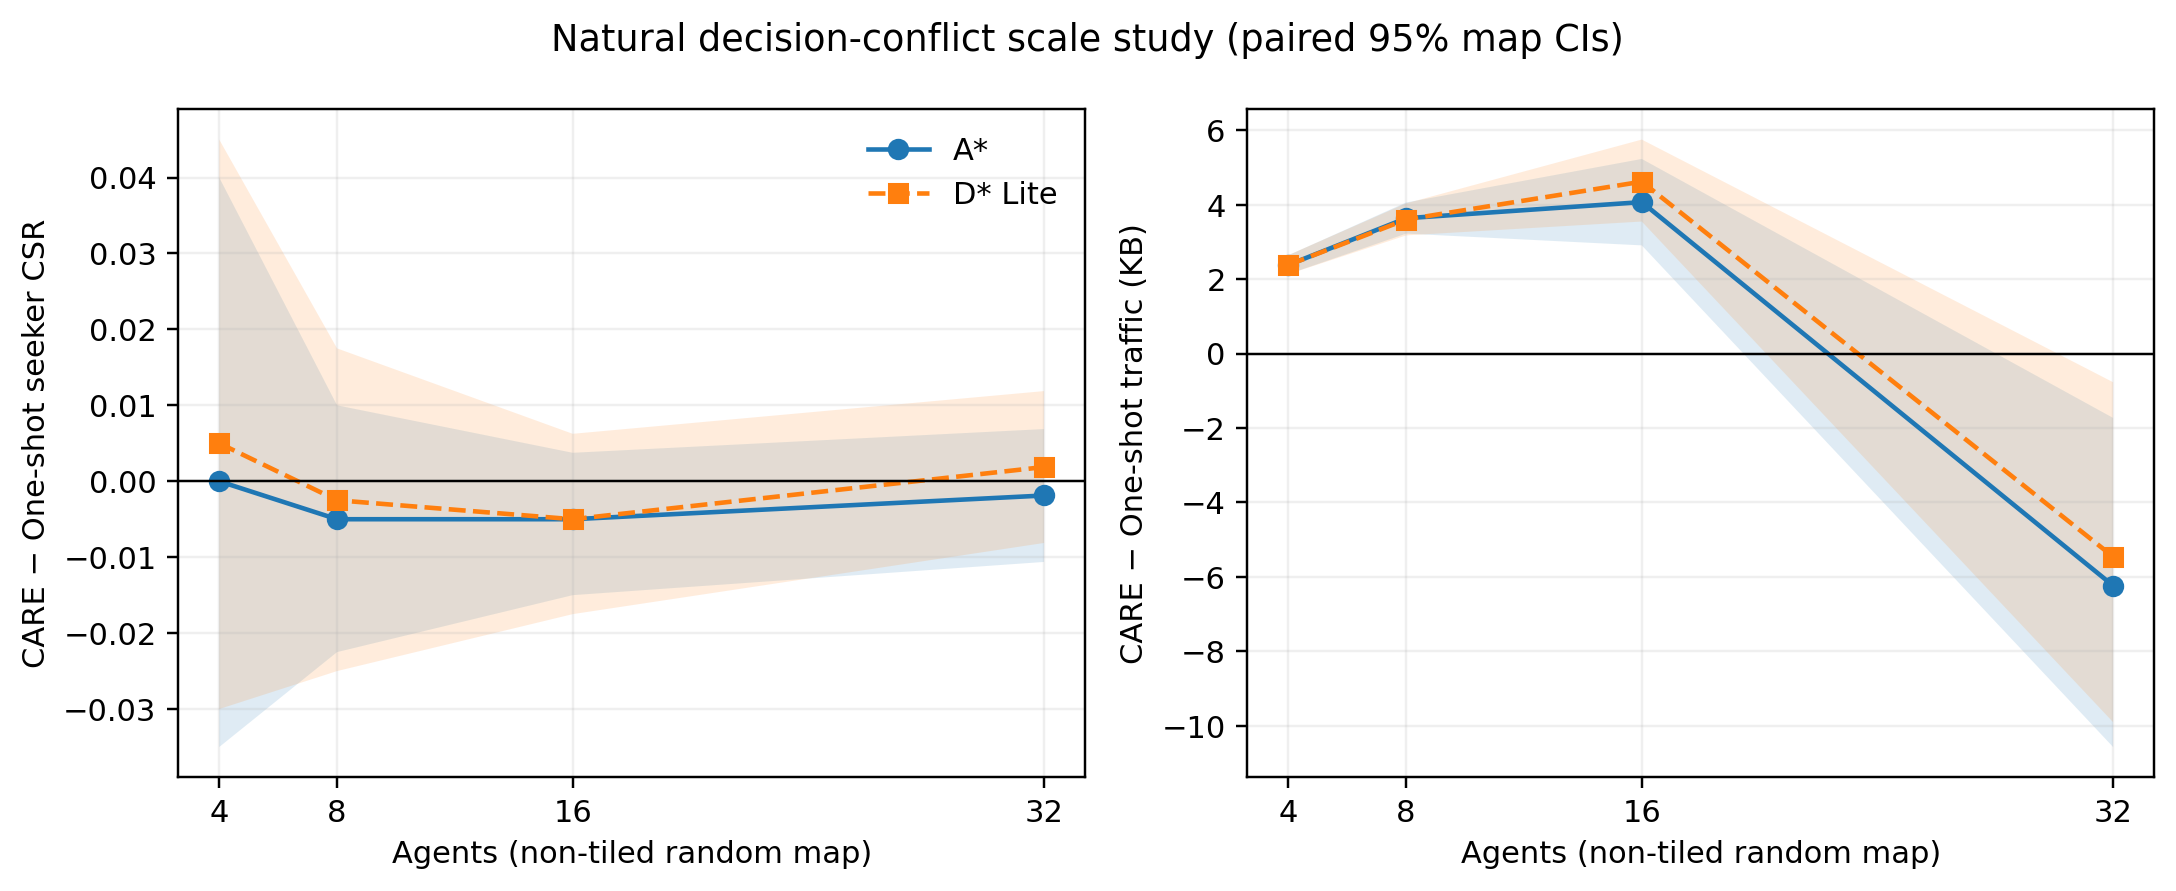
\includegraphics[width=\columnwidth]{care_natural_scale.png}
 \caption{Paired CARE-minus-One-shot effects on non-tiled natural maps. Shading
 is the map-bootstrap 95\% CI; every seeker-CSR interval crosses zero.}
 \label{fig:natural-scale}
\end{figure}

Exact certification also has measurable compute cost because up to 37
scenarios and 256 candidate subsets are evaluated online. The caps make the
optimization finite and auditable, but do not make it negligible. This
tradeoff, the frequent paired intervals that include zero against simpler
controls, conditioning on the natural-suite predicate bundle, finite 25-step controlled horizon,
and the common controlled decision template are the principal limitations.

\section{Conclusion}
CARE formulates explicit-map repair as minimum encoded-query separation of all
deadline-feasible action conflicts in a bounded sparse scenario family. The
certificate is exact within that model and improves seeker reliability at low
additional traffic on controlled multifork tasks. Closest-work adaptations,
the rejected route-slack gate, and non-tiled natural maps prevent a broader
claim: much of the gain comes from task awareness, and no general natural-map
advantage is detected. The supported contribution is therefore a precise,
auditable decision-certificate objective and solver---not a learned policy,
an unrestricted guarantee, or a universal replacement for reliable delivery.

\bibliographystyle{IEEEtran}
\bibliography{psr_icassp_refs}
\end{document}
